%{{第八十回}}{第八十回}}

\chapter{薛文龙悔娶河东狮\hspace{.5em}贾迎春误嫁中山狼(续)}

{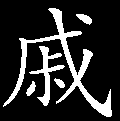
\includegraphics[width=3mm]{../Images/00005}\kaishu 叙桂花妒用实笔,叙孙家恶用虚笔;叙宝玉卧病是省笔,叙宝玉烧香是停笔。}

话说金桂听了,将脖项一扭,嘴唇一撇,{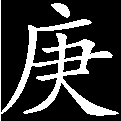
\includegraphics[width=3mm]{../Images/00004}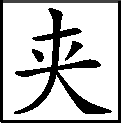
\includegraphics[width=3mm]{../Images/00012}\footnotesize \kaishu 画出一个悍妇来。}鼻孔里哧哧两声,{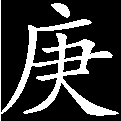
\includegraphics[width=3mm]{../Images/00004}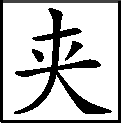
\includegraphics[width=3mm]{../Images/00012}\footnotesize \kaishu 真真追魂摄魄之笔。}拍着掌冷笑道:``菱角花谁闻见香来着?若说菱角香了,正经那些香花放在那里?可是不通之极!''香菱道:``不独菱角花,就连荷叶莲蓬,都是有一股清香的。但他那原不是花香可比,若静日静夜或清早半夜细领略了去,那一股香比是花儿都好闻呢。就连菱角、鸡头、苇叶、芦根得了风露,那一股清香,就令人心神爽快的。''{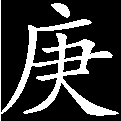
\includegraphics[width=3mm]{../Images/00004}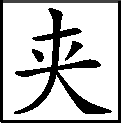
\includegraphics[width=3mm]{../Images/00012}\footnotesize \kaishu 说的出便是慧心人,何况菱卿哉?}金桂道:``依你说,那兰花桂花倒香的不好了?''{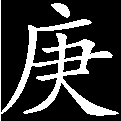
\includegraphics[width=3mm]{../Images/00004}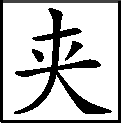
\includegraphics[width=3mm]{../Images/00012}\footnotesize \kaishu 又陪一个兰花,一则是自高声价,二则是诱人犯法。}香菱说到热闹头上,忘了忌讳,便接口道:``兰花桂花的香,又非别花之香可比。''一句未完,金桂的丫鬟名唤宝蟾者,忙指着香菱的脸儿说道:``要死,要死!你怎么真叫起姑娘的名字来!''香菱猛省了,反不好意思,忙陪笑赔罪说:``一时说顺了嘴,奶奶别计较。''金桂笑道:``这有什么,你也太小心了。但只是我想这个`香'字到底不妥,意思要换一个字,不知你服不服?''香菱忙笑道:``奶奶说那里话,此刻连我一身一体俱属奶奶,何得换一名字反问我服不服,叫我如何当得起。奶奶说那一个字好,就用那一个。''金桂笑道:``你虽说的是,只怕姑娘多心,说:`我起的名字,反不如你?你能来了几日,就驳我的回了。'''香菱笑道:``奶奶有所不知,当日买了我来时,原是老奶奶使唤的,故此姑娘起得名字。后来我自伏侍了爷,就与姑娘无涉了。如今又有了奶奶,益发不与姑娘相干。况且姑娘又是极明白的人,如何恼得这些呢。''金桂道:``既这样说,`香'字竟不如`秋'字妥当。菱角菱花皆盛于秋,岂不比`香'字有来历些。''香菱道:``就依奶奶这样罢了。''自此后遂改了秋字,宝钗亦不在意。

只因薛蟠天性是``得陇望蜀''的,如今得娶了金桂,又见金桂的丫鬟宝蟾有三分姿色,举止轻浮可爱,便时常要茶要水的故意撩逗他。宝蟾虽亦解事,只是怕着金桂,不敢造次,且看金桂的眼色。金桂亦颇觉察其意,想着:``正要摆布香菱,无处寻隙,如今他既看上了宝蟾,如今且舍出宝蟾去与他,他一定就和香菱疏远了,我且乘他疏远之时,便摆布了香菱。那时宝蟾原是我的人,也就好处了。''打定了主意,伺机而发。

这日薛蟠晚间微醺,又命宝蟾倒茶来吃。薛蟠接碗时,故意捏他的手。宝蟾又乔装躲闪,连忙缩手。两下失误,``豁啷''一声,茶碗落地,泼了一身一地的茶。薛蟠不好意思,佯说宝蟾不好生拿着。宝蟾说:``姑爷不好生接。''金桂冷笑道:``两个人的腔调儿都够使了。别打量谁是傻子。''薛蟠低头微笑不语,宝蟾红了脸出去。一时安歇之时,金桂便故意的撵薛蟠别处去睡,``省得你馋痨饿眼。''薛蟠只是笑。金桂道:``要作什么和我说,别偷偷摸摸的不中用。''薛蟠听了,仗着酒盖脸,便趁势跪在被上拉着金桂笑道:``好姐姐,你若要把宝蟾赏了我,你要怎样就怎样。你要人脑子也弄来给你。''金桂笑道:``这话好不通。你爱谁,说明了,就收在房里,省得别人看着不雅。我可要什么呢。''薛蟠得了这话,喜的称谢不尽,是夜\elegantpar{曲尽丈夫之道}{大约是政老所云,奶奶奶奶},{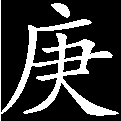
\includegraphics[width=3mm]{../Images/00004}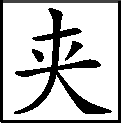
\includegraphics[width=3mm]{../Images/00012}\footnotesize \kaishu ``曲尽丈夫之道'',奇闻奇语。}奉承金桂。次日也不出门,只在家中厮奈,越发放大了胆。

至午后,金桂故意出去,让个空儿与他二人。薛蟠便拉拉扯扯的起来。宝蟾心里也知八九,也就半推半就,正要入港。谁知金桂是有心等候的,料必在难分之际,便叫丫头小舍儿过来。原来这小丫头也是金桂从小儿在家使唤的,因他自幼父母双亡,无人看管,便大家叫他作小舍儿,专作些粗笨的生活。{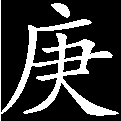
\includegraphics[width=3mm]{../Images/00004}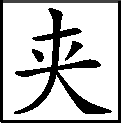
\includegraphics[width=3mm]{../Images/00012}\footnotesize \kaishu 铺叙小舍儿首尾,忙中又点``薄命''二字,与痴丫头遥遥作对。}金桂如今有意独唤他来吩咐道:``你去告诉秋菱,到我屋里将手帕取来,不必说我说的。''{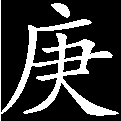
\includegraphics[width=3mm]{../Images/00004}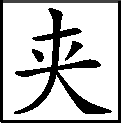
\includegraphics[width=3mm]{../Images/00012}\footnotesize \kaishu 金桂坏极!所以独使小舍为此。}小舍儿听了,一径寻着香菱说:``菱姑娘,奶奶的手帕子忘记在屋里了。你去取来送上去岂不好?''香菱正因金桂近日每每的折挫他,不知何意,百般竭力挽回不暇。{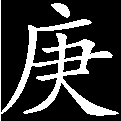
\includegraphics[width=3mm]{../Images/00004}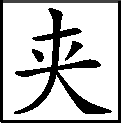
\includegraphics[width=3mm]{../Images/00012}\footnotesize \kaishu 总为痴心人一哭。}听了这话,忙往房里来取。不防正遇见他二人推就之际,一头撞了进去,自己倒羞的耳面飞红,忙转身回避不迭。那薛蟠自为是过了明路的,除了金桂,无人可怕,所以连门也不掩,今见香菱撞来,故也略有些惭愧,还不十分在意。无奈宝蟾素日最是说嘴要强的,今遇见了香菱,便恨无地缝儿可入,忙推开薛蟠,一径跑了,口内还恨怨不迭,说他强奸力逼等语。薛蟠好容易圈哄的要上手,却被香菱打散,不免一腔兴头变作了一腔恶怒,都在香菱身上,不容分说,赶出来啐了两口,骂道:``死娼妇,你这会子作什么来撞尸游魂!''香菱料事不好,三步两步早已跑了。薛蟠再来找宝蟾,已无踪迹了,于是恨的只骂香菱。

至晚饭后,已吃得醺醺然,洗澡时不防水略热了些,烫了脚,便说香菱有意害他,\elegantpar{赤条精光赶着香菱踢打了两下}{薛总如此}。香菱虽未受过这气苦,既到此时,也说不得了,只好自悲自怨,各自走开。

彼时金桂已暗和宝蟾说明,今夜令薛蟠和宝蟾在香菱房中去成亲,命香菱过来陪自己先睡。先是香菱不肯,金桂说他嫌脏了,再必是图安逸,怕夜里劳动伏侍,又骂说:``你那没见世面的主子,见一个,爱一个,把我的人霸占了去,又不叫你来。到底是什么主意,想必是逼我死罢了。''薛蟠听了这话,又怕闹黄了宝蟾之事,忙又赶来骂香菱:``不识抬举!再不去便要打了!''香菱无奈,只得抱了铺盖来。金桂命他在地下铺睡。香菱无奈,只得依命。刚睡下,便叫倒茶,一时又叫捶腿,如是一夜七八次,总不使其安逸稳卧片时。那薛蟠得了宝蟾,如获珍宝,一概都置之不顾。恨的金桂暗暗的发恨道:``且叫你乐这几天,等我慢慢的摆布了来,那时可别怨我!''一面隐忍,一面设计摆布香菱。

半月光景,忽又装起病来,只说心疼难忍,四肢不能转动。{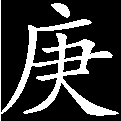
\includegraphics[width=3mm]{../Images/00004}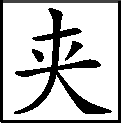
\includegraphics[width=3mm]{../Images/00012}\footnotesize \kaishu 半月工夫,诸计安矣。}请医疗治不效,众人都说是香菱气的。闹了两日,忽又从金桂的枕头内抖出纸人来,上面写着金桂的年庚八字,有五根针钉在心窝并四肢骨节等处。于是众人反乱起来,当作新闻,先报与薛姨妈。薛姨妈先忙手忙脚的,薛蟠自然更乱起来,立刻要拷打众人。金桂笑道:``何必冤枉众人,大约是宝蟾的镇魇法儿。''{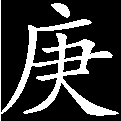
\includegraphics[width=3mm]{../Images/00004}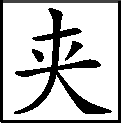
\includegraphics[width=3mm]{../Images/00012}\footnotesize \kaishu 恶极!坏极!}薛蟠道:``他这些时并没多空儿在你房里,何苦赖好人。''{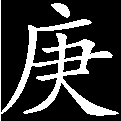
\includegraphics[width=3mm]{../Images/00004}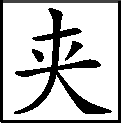
\includegraphics[width=3mm]{../Images/00012}\footnotesize \kaishu 正要老兄此句。}金桂冷笑道:``除了他还有谁,莫不是我自己不成!虽有别人,谁可敢进我的房呢。''薛蟠道:``香菱如今是天天跟着你,他自然知道,先拷问他就知道了。''金桂冷笑道:``拷问谁,谁肯认?依我说竟装个不知道,大家丢开手罢了。横竖治死我也没什么要紧,乐得再娶好的。若据良心上说,左不过你三个多嫌我一个。''说着,一面痛哭起来。

薛蟠更被这一席话激怒,\elegantpar{顺手抓起一根门闩来}{前文打宝玉,他还发了疯},{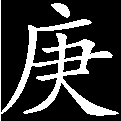
\includegraphics[width=3mm]{../Images/00004}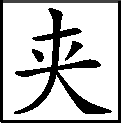
\includegraphics[width=3mm]{../Images/00012}\footnotesize \kaishu 与前要打死宝玉遥遥一对。}一径抢步找着香菱,不容分说便劈头劈面打起来,一口咬定是香菱所施。香菱叫屈,薛姨妈跑来禁喝说:``不问明白,你就打起人来了。这丫头伏侍了你这几年,那一点不周到,不尽心?他岂肯如今作这没良心的事!你且问个清浑皂白,再动粗卤。''金桂听见他婆婆如此说着,怕薛蟠耳软心活,便益发嚎啕大哭起来,一面又哭喊说:``这半个多月把我的宝蟾霸占了去,不容他进我的房,唯有秋菱跟着我睡。我要拷问宝蟾,你又护到头里。你这会子又赌气打他去。治死我,再拣富贵的标致的娶来就是了,何苦作出这些把戏来!''薛蟠听了这些话,越发着了急。薛姨妈听见金桂句句挟制着儿子,百般恶赖的样子,十分可恨。无奈儿子偏不硬气,已是被他挟制软惯了。如今又勾搭上丫头,被他说霸占了去,他自己反要占温柔让夫之礼。这魇魔法究竟不知谁作的,实是俗语说的``清官难断家务事'',此事正是公婆难断床帏事了。因此无法,只得赌气喝骂薛蟠说:``不争气的孽障!骚狗也比你体面些!谁知你三不知的把陪房丫头也摸索上了,叫老婆说嘴霸占了丫头,什么脸出去见人!也不知谁使的法子,也不问青红皂白,好歹就打人。我知道你是个得新弃旧的东西,白辜负了我当日的心。他既不好,你也不许打,我立即叫人牙子来卖了他,你就心净了。''说着,命香菱``收拾了东西跟我来'',一面叫人``去,快叫个人牙子来,多少卖几两银子,拔去肉中刺,眼中钉,大家过太平日子。''

薛蟠见母亲动了气,早也低下头了。金桂听了这话,便隔着窗子往外哭道:``你老人家只管卖人,不必说着一个扯着一个的。我们狠是那吃醋拈酸容不下人的不成,怎么`拔出肉中刺,眼中钉'?是谁的钉,谁的刺?但凡多嫌着他,也不肯把我的丫头也收在房里了。''薛姨妈听说,气的身战气咽道:``这是谁家的规矩?婆婆这里说话,媳妇隔着窗子拌嘴。亏你是旧家人家的女儿!满嘴里大呼小喊,说的是些什么!''薛蟠急的跺脚说:``罢哟,罢哟!看人听见笑话。''金桂意谓一不作,二不休,越发发泼喊起来了,说:``我不怕人笑话!你的小老婆治我害我,我倒怕人笑话了!再不然,留下他,就卖了我。谁还不知道你薛家有钱,行动拿钱垫人,又有好亲戚挟制着别人。你不趁早施为,还等什么?嫌我不好,谁叫你们瞎了眼,三求四告的跑了我们家作什么去了!这会子人也来了,金的银的也赔了,略有个眼睛鼻子的也霸占去了,该挤发我了!''一面哭喊,一面滚揉,自己拍打。薛蟠急的说又不好,劝又不好,打又不好,央告又不好,只是出入咳声叹气,抱怨说运气不好。{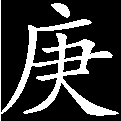
\includegraphics[width=3mm]{../Images/00004}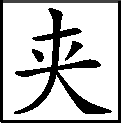
\includegraphics[width=3mm]{../Images/00012}\footnotesize \kaishu 果然不差。}

当下薛姨妈早被薛宝钗劝进去了,只命人来卖香菱。宝钗笑道:``咱们家从来只知买人,并不知卖人之说。妈可是气的糊涂了,倘或叫人听见,岂不笑话。哥哥嫂子嫌他不好,留下我使唤,我正也没人使呢。''薛姨妈道:``留着他还是淘气,不如打发了他倒干净。''宝钗笑道:``他跟着我也是一样,横竖不叫他到前头去。从此断绝了他那里,也如卖了一般。''香菱早已跑到薛姨妈跟前痛哭哀求,只不愿出去,情愿跟着姑娘,薛姨妈也只得罢了。

自此以后,香菱果跟随宝钗去了,把前面路径竟一心断绝。虽然如此,终不免对月伤悲,挑灯自叹。本来怯弱,虽在薛蟠房中几年,皆由血分中有病,是以并无胎孕。今复加以气怒伤感,内外折挫不堪,竟酿成干血之症,日渐羸瘦作烧,饮食懒进,请医诊视服药亦不效验。那时金桂又吵闹了数次,气的薛姨妈母女惟暗自垂泪,怨命而已。薛蟠虽曾仗着酒胆挺撞过两三次,持棍欲打,那金桂便递与他身子随意叫打;这里持刀欲杀时,便伸与他脖项。薛蟠也实不能下手,只得乱闹了一阵罢了。如今习惯成自然,反使金桂越发长了威风,薛蟠越发软了气骨。虽是香菱犹在,却亦如不在的一般,虽不能十分畅快,就不觉的碍眼了,且姑置不究。

如今又渐次寻趁宝蟾。宝蟾却不比香菱的情性,最是个烈火干柴,既和薛蟠情投意合,便把金桂忘在脑后。{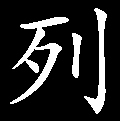
\includegraphics[width=3mm]{../Images/00007}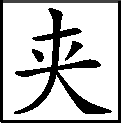
\includegraphics[width=3mm]{../Images/00012}\footnotesize \kaishu 妙!所谓天理还报不爽。}近见金桂又作践他,他便不肯服低容让半点。先是一冲一撞的拌嘴,后来金桂气急了,甚至于骂,再至于打。他虽不敢还言还手,便大撒泼性,拾头打滚,寻死觅活,昼则刀剪,夜则绳索,无所不闹。薛蟠此时一身难以两顾,惟徘徊观望于二者之间,十分闹的无法,便出门躲在外厢。金桂不发作性气,有时欢喜,便纠聚人来斗纸牌、掷骰子作乐。又生平最喜啃骨头,每日务要杀鸡鸭,将肉赏人吃,只单以油炸焦骨头下酒。吃的不奈烦或动了气,便肆行海骂,说:``有别的忘八粉头乐的,我为什么不乐!''薛家母女总不去理他。薛蟠亦无别法,惟日夜悔恨不该娶这搅家星罢了,都是一时没了主意。{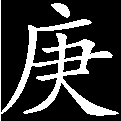
\includegraphics[width=3mm]{../Images/00004}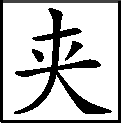
\includegraphics[width=3mm]{../Images/00012}\footnotesize \kaishu 补足本题。}于是宁荣二宅之人,上上下下,无有不知,无有不叹者。

此时宝玉已过了百日,出门行走。亦曾过来见过金桂,``举止形容也不怪厉,一般是鲜花嫩柳,与众姊妹不差上下的人,焉得这等样情性,可为奇之至极''。{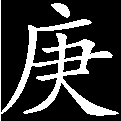
\includegraphics[width=3mm]{../Images/00004}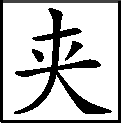
\includegraphics[width=3mm]{../Images/00012}\footnotesize \kaishu 别书中形容妒妇,必曰``黄发黧面'',岂不可笑?}因此心下纳闷。这日与王夫人请安去,又正遇见迎春奶娘来家请安,说起孙绍祖甚属不端,``姑娘惟有背地里淌眼抹泪的,只要接了来家散诞两日''。王夫人因说:``我正要这两日接他去,只因七事八事的都不遂心,{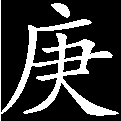
\includegraphics[width=3mm]{../Images/00004}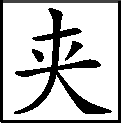
\includegraphics[width=3mm]{../Images/00012}\footnotesize \kaishu 草蛇灰线,后文方不见突然。}所以就忘了。前儿宝玉去了,回来也曾说过的。{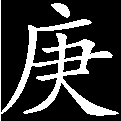
\includegraphics[width=3mm]{../Images/00004}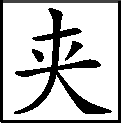
\includegraphics[width=3mm]{../Images/00012}\footnotesize \kaishu 补明。}明日是个好日子,就接去。''正说着,贾母打发人来找宝玉,说:``明儿一早往天齐庙还愿。''宝玉如今巴不得各处去逛逛,听见如此,喜的一夜不曾合眼,盼明不明的。

次日一早,梳洗穿戴已毕,随了两三个老嬷嬷坐车出西城门外天齐庙来烧香还愿。这庙里已是昨日预备停妥的。宝玉天生性怯,不敢近狰狞神鬼之像。这天齐庙本系前朝所修,极其宏壮。如今年深岁久,又极其荒凉。里面泥胎塑像皆极其凶恶,是以忙忙的焚过纸马钱粮,便退至道院歇息。一时吃过饭,众嬷嬷和李贵等人围随宝玉到处散诞顽耍了一回。宝玉困倦,复回至静室安歇。众嬷嬷生恐他睡着了,便请当家的老王道士来陪他说话儿。这老王道士专意在江湖上卖药,弄些海上方治人射利,这庙外现挂着招牌,丸散膏丹,色色俱备,亦长在宁荣两宅走动熟惯,都与他起了个浑号,唤他作``王一贴'',言他的膏药灵验,只一贴百病皆除之意。当下王一贴进来,宝玉正歪在炕上想睡,李贵等正说``哥儿别睡着了'',厮混着。看见王一贴进来,都笑道:``来的好,来的好。王师父,你极会说古记的,说一个与我们小爷听听。''王一贴笑道:``正是呢。哥儿别睡,仔细肚里面筋作怪。''说着,满屋里人都笑了。{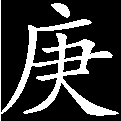
\includegraphics[width=3mm]{../Images/00004}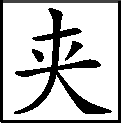
\includegraphics[width=3mm]{../Images/00012}\footnotesize \kaishu 王一贴又与张道士遥遥一对,特犯不犯。}

宝玉也笑着起身整衣。王一贴喝命徒弟们快泡好酽茶来。茗烟道:``我们爷不吃你的茶,连这屋里坐着还嫌膏药气息呢。''王一贴笑道:``没当家花花的,膏药从不拿进这屋里来的。知道哥儿今日必来,头三五天就拿香熏了又熏的。''宝玉道:``可是呢,天天只听见你的膏药好,到底治什么病?''王一贴道:``哥儿若问我的膏药,说来话长,其中细理,一言难尽。共药一百二十味,君臣相济,宾主得宜,温凉兼用,贵贱殊方。内则调元补气,开胃口,养荣卫,宁神安志,去寒去暑,化食化痰;外则和血脉,舒筋络,出死肌,生新肉,去风散毒。其效如神,贴过的便知。''宝玉道:``我不信一张膏药就治这些病。我且问你,倒有一种病可也贴的好么?''王一贴道:``百病千灾,无不立效。若不见效,哥儿只管揪着胡子打我这老脸,拆我这庙何如?只说出病源来。''宝玉笑道:``你猜,若你猜的着,便贴的好了。''王一贴听了,寻思一会,笑道:``这倒难猜,只怕膏药有些不灵了。''宝玉命李贵等:``你们且出去散散。这屋里人多,越发蒸臭了。''李贵等听说,且都出去自便,只留下茗烟一人。这茗烟手内点着一枝梦甜香,{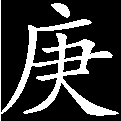
\includegraphics[width=3mm]{../Images/00004}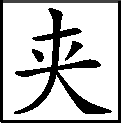
\includegraphics[width=3mm]{../Images/00012}\footnotesize \kaishu 与前文一照。}宝玉命他坐在身旁,却倚在他身上。王一贴心有所动,{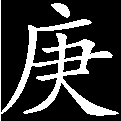
\includegraphics[width=3mm]{../Images/00004}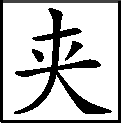
\includegraphics[width=3mm]{../Images/00012}\footnotesize \kaishu 四字好。万端生于心,心邪则意在于财。}便笑嘻嘻走近前来,悄悄的说道:``我可猜着了。想是哥儿如今有了房中的事情,要滋助的药,可是不是?''话犹未完,茗烟先喝道:``该死,打嘴!''宝玉\elegantpar{犹未解}{对“尚出神”看},{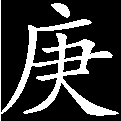
\includegraphics[width=3mm]{../Images/00004}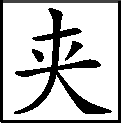
\includegraphics[width=3mm]{../Images/00012}\footnotesize \kaishu ``未解''妙!若解则不成文矣。}忙问:``他说什么?''茗烟道:``信他胡说。''唬的王一贴不敢再问,只说:``哥儿明说了罢。''

宝玉道:``我问你,可有贴女人的妒病方子没有?''{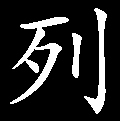
\includegraphics[width=3mm]{../Images/00007}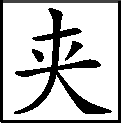
\includegraphics[width=3mm]{../Images/00012}\footnotesize \kaishu 千古奇文奇语,仍归结至上半回正文,细密如此。}王一贴听说,拍手笑道:``这可罢了。不但说没有方子,就是听也没有听见过。''宝玉笑道:``这样还算不得什么。''王一贴又忙道:``这贴妒的膏药倒没经过,倒有一种汤药或者可医,只是慢些儿,不能立竿见影的效验。''宝玉道:``什么汤药,怎么吃法?''王一贴道:``\elegantpar{这叫做`疗妒汤':用极好的秋梨一个,二钱冰糖,一钱陈皮,水三碗,梨熟为度,每日清早吃这么一个梨,吃来吃去就好了。}{好吃好吃}''宝玉道:``这也不值什么,只怕未必见效。''王一贴道:``\elegantpar{一剂不效吃十剂,今日不效明日再吃,今年不效吃到明年。横竖这三味药都是润肺开胃不伤人的,甜丝丝的,又止咳嗽,又好吃。吃过一百岁,人横竖是要死的,死了还妒什么!那时就见效了。}{见效见效,神医神医}''{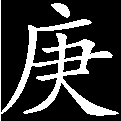
\includegraphics[width=3mm]{../Images/00004}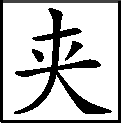
\includegraphics[width=3mm]{../Images/00012}\footnotesize \kaishu 此科诨一收,方为奇趣之至。}说着,宝玉茗烟都大笑不止,骂``油嘴的牛头''。王一贴笑道:``不过是闲着解午盹罢了,有什么关系。说笑了你们就值钱。实告你们说,连膏药也是假的。我有真药,我还吃了作神仙呢。有真的,跑到这里来混?''{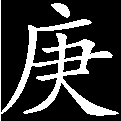
\includegraphics[width=3mm]{../Images/00004}\includegraphics[width=3mm]{../Images/00012}\footnotesize \kaishu 寓意深远,在此数语。}正说着,吉时已到,请宝玉出去焚化钱粮散福。功课完毕,方进城回家。

那时,迎春已来家好半日,孙家的婆娘媳妇等人已待过晚饭,打发回家去了。迎春方哭哭啼啼的在王夫人房中诉委曲,说孙绍祖``一味好色,好赌酗酒,家中所有的媳妇丫头将及淫遍。略劝过两三次,便骂我是`醋汁子老婆拧出来的'。{\includegraphics[width=3mm]{../Images/00004}\includegraphics[width=3mm]{../Images/00012}\footnotesize \kaishu 奇文奇骂。为迎春一哭,又为荣府一哭。◇恨薛蟠何等刚霸,偏不能以此语及金桂,使人忿忿。此书中全是不平,又全是意外之料\href{../Text/part0084_split_000.html\#lnkback_2_a}{\textsuperscript{②}}。}又说老爷曾收着他五千银子,不该使了他的。如今他来要了两三次不得,他便指着我的脸说道:`你别和我充夫人娘子,你老子使了我五千银子,把你准折卖给我的。好不好,打一顿撵在下房里睡去。当日有你爷爷在时,希图上我们的富贵,赶着相与的。论理我和你父亲是一辈,如今强压我的头,卖了一辈。又不该作了这门亲,倒没的叫人看着赶势利似的。'''{\includegraphics[width=3mm]{../Images/00004}\includegraphics[width=3mm]{../Images/00012}\footnotesize \kaishu 不通,可笑。遁辞如闻。}一行说,一行哭的呜呜咽咽,连王夫人并众姊妹无不落泪。王夫人只得用言语解劝说:``已是遇见了这不晓事的人,可怎么样呢。想当日你叔叔也曾劝过大老爷,不叫作这门亲的。大老爷执意不听,一心情愿,到底作不好了。我的儿,这也是你的命。''迎春哭道:``我不信!我的命就这么不好了么?从小儿没了娘,幸而过婶子这边过了几年心净日子,如今偏又是这么个结果!''

王夫人一面解劝,一面问他随意要在那里安歇。迎春道:``乍乍的离了姊妹们,只是眠思梦想。二则还记挂着我的屋子,还得在园里旧房子里住得三五天,死也甘心了。不知下次还可能得住不得住了呢!''王夫人忙劝道:``快休乱说。不过年轻的夫妻们,闲牙斗齿,亦是万万人之常事,何必说这丧话。''仍命人忙忙的收拾紫菱洲房屋,命姊妹们陪伴着解释,又吩咐宝玉:``不许在老太太跟前走漏一些风声,倘或老太太知道了这些事,都是你说的。''宝玉唯唯的听命。迎春是夕仍在旧馆安歇。众姊妹等更加亲热异常。

一连住了三日,才往邢夫人那边去。先辞过贾母及王夫人,然后与众姊妹分别,更皆悲伤不舍。还是王夫人薛姨妈等安慰劝释,方止住了过那边去。{\includegraphics[width=3mm]{../Images/00004}\includegraphics[width=3mm]{../Images/00012}\footnotesize \kaishu 凡迎春之文皆从宝玉眼中写出。前``悔娶河东狮''是实写,``误嫁中山狼''出迎春口中可为虚写,以虚虚实实变幻体格,各尽其法。}又在邢夫人处住了两日,就有孙绍祖的人来接去。迎春虽不愿去,无奈惧孙绍祖之恶,只得勉强忍情作辞去了。邢夫人本不在意,也不问其夫妻和睦,家务烦难,只面情塞责而已。终不知端的,且听下回分解。

{\includegraphics[width=3mm]{../Images/00005}\kaishu 总评:此文一为择婿者说法,一为择妻者说法。择婿者必以得人物轩昂、家道丰厚、荫袭公子为快,择妻者必以得容貌艳丽、妆奁富厚、子女盈门为快,殊不知``以貌取人,失之子羽''。试看桂花夏家、指挥孙家,何等可羡可乐。卒至迎春含悲,薛蟠贻恨,可慨也夫!}

% {\href{../Text/part0084_split_000.html\#navto_1_a}{①}按:列藏本第七十九回包含了诸本第七十九和第八十回的全部内容,应为原稿面貌。底本虽已分回但第八十回缺回目,因第七十九回回目已概括了两回内容,本回不采用后人所拟的回目。}

% {\href{../Text/part0084_split_000.html\#navto_2_a}{②}``意外之料'',列本批语同。自俞平伯先生校改为``意料之外'',今人多从之。按本书中虽有使用``意料之外''这一词组,但不能因此认为``意外之料''为错。试观其近义词``意外之想'',在书中就和``意想之外''并用,且前者出现次数还要多些。}
